\documentclass[a4paper,12pt]{article}

\usepackage[utf8x]{inputenc}   % omogoča uporabo slovenskih črk kodiranih v formatu UTF-8
\usepackage[slovene,english]{babel}    % naloži, med drugim, slovenske delilne vzorce
\usepackage[pdftex]{graphicx}  % omogoča vlaganje slik različnih formatov
\usepackage{fancyhdr}          % poskrbi, na primer, za glave strani
\usepackage{amssymb}           % dodatni simboli
\usepackage{amsmath}           % eqref, npr.
%\usepackage{hyperxmp}
\usepackage[hyphens]{url}  % dodal Solina
\usepackage{comment}       % dodal Solina

\usepackage[pdftex, colorlinks=true,
						citecolor=black, filecolor=black, 
						linkcolor=black, urlcolor=black,
						pagebackref=false, 
						pdfproducer={LaTeX}, pdfcreator={LaTeX}, hidelinks]{hyperref}

\usepackage{color}       % dodal Solina
\usepackage{soul}       % dodal Solina
\usepackage{indentfirst}

\usepackage{graphicx}
\usepackage[figurename=Slika]{caption}


% Page setup
\usepackage{geometry}

\geometry{top=2.5cm, bottom=2.5cm, left=2.5cm, right=2.5cm}

\title{\vspace{-4cm}Seminarska naloga za Računalniško grafiko\\[0.5cm] \huge \textbf{Frodo's Nightmares} \vspace{-1cm}}
\author{Tim Thuma (63230333), Tilen Medved (63230207), Luka Hribar (63230109)}

\newcommand{\BibTeX}{{\sc Bib}\TeX}

%%%%%%%%%%%%%%%%%%%%%%%%%%%%%%%%%%%%%%%%
%	DIPLOMA INFO
%%%%%%%%%%%%%%%%%%%%%%%%%%%%%%%%%%%%%%%%
\newcommand{\ttitle}{Frodo's Nightmares}
\newcommand{\tsubject}{\ttitle}
\newcommand{\tauthor}{Tim Thuma (63230333), Tilen Medved (63230207), Luka Hribar (63230109)}


%%%%%%%%%%%%%%%%%%%%%%%%%%%%%%%%%%%%%%%%
%	HYPERREF SETUP
%%%%%%%%%%%%%%%%%%%%%%%%%%%%%%%%%%%%%%%%
\hypersetup{pdftitle={\ttitle}}
\hypersetup{pdfsubject=\ttitle}
\hypersetup{pdfauthor={\tauthor}}

\def\Title{\ttitle}
\def\Author{\tauthor}


\newcommand{\autfont}{\Large}
\newcommand{\titfont}{\LARGE\bf}
\newcommand{\clearemptydoublepage}{\newpage{\pagestyle{empty}\cleardoublepage}}
\setcounter{tocdepth}{1}	      % globina kazala

\def\convertDate{%
    \getYear
}

{\catcode`\D=12
 \gdef\getYear D:#1#2#3#4{\edef\xYear{#1#2#3#4}\getMonth}
}
\def\getMonth#1#2{\edef\xMonth{#1#2}\getDay}
\def\getDay#1#2{\edef\xDay{#1#2}\getHour}
\def\getHour#1#2{\edef\xHour{#1#2}\getMin}
\def\getMin#1#2{\edef\xMin{#1#2}\getSec}
\def\getSec#1#2{\edef\xSec{#1#2}\getTZh}
\def\getTZh +#1#2{\edef\xTZh{#1#2}\getTZm}
\def\getTZm '#1#2'{%
    \edef\xTZm{#1#2}%
    \edef\convDate{\xYear-\xMonth-\xDay T\xHour:\xMin:\xSec+\xTZh:\xTZm}%
}

\expandafter\convertDate\pdfcreationdate 

%%%%%%%%%%%%%%%%%%%%%%%%%%%%%%%%%%%%%%%%
% get pdftex version string
%%%%%%%%%%%%%%%%%%%%%%%%%%%%%%%%%%%%%%%% 
\newcount\countA
\countA=\pdftexversion
\advance \countA by -100
\def\pdftexVersionStr{pdfTeX-1.\the\countA.\pdftexrevision}


%%%%%%%%%%%%%%%%%%%%%%%%%%%%%%%%%%%%%%%%
% pdfInfo
%%%%%%%%%%%%%%%%%%%%%%%%%%%%%%%%%%%%%%%%  
\pdfinfo{%
    /Title    (\ttitle)
    /Author   (\tauthor)
    /Subject  (\ttitle)
    /ModDate  (\pdfcreationdate)
    /Trapped  /False
}





\begin{document}

\thispagestyle{empty}%
\begin{center}
 {\large\sc Univerza v Ljubljani\\%
   Fakulteta za računalništvo in informatiko}%
 \vskip 10em%
 {\autfont Tim Thuma (63230333), Tilen Medved (63230207),\\Luka Hribar (63230109) \par}%
 {\vskip 1em \titfont Frodo's Nightmares \par}%
 {\vskip 3em \textsc{SEMINARSKA NALOGA PRI PREDMETU RAČUNALNIŠKA GRAFIKA\\[5mm]
   VISOKOŠOLSKI STROKOVNI ŠTUDIJSKI PROGRAM\\ PRVE STOPNJE\\ RAČUNALNIŠTVO IN INFORMATIKA}\par}
 \vfill\null
 {\large \textsc{Mentor}: izr. prof. dr. Iztok Lebar Bajec \par}%
 {\vskip 2em \large Ljubljana, januar 2025 \par}%
\end{center}


\newpage

\section*{\textit{Abstract}}

\noindent V okviru seminarske naloge za predmet Računalniška grafika smo ustvarili igro ugankarskega žanra z naslovom Frodo’s Nightmares. Igra je napisana v programskem jeziku Javascript in za delovanje uporablja WebGPU vmesnik. Glavni osebek Frodo je postavljen v sceno hiše iz katere mora pobegniti tako, da rešuje uganke. Uganke so sestavljene iz različnih interakcij z objekti, postavljenimi po hiši, na koncu pa mora igralec pobrati ključ, ki odpre izhodna vrata. Scena je realistična, toda poenostavljena za lažje delo. Kamera na igralca gleda iz tretjeosebnega položaja in se premika skupaj s Frodom. Pri kameri gre za perspektivno projekcijo. V sceni je več luči, najpomembnejši pa sta petrolejka in ročna svetilka, s katerima Frodo osvetljuje prostor okoli sebe. Za osvetlitev smo uporabili Blinn-Phongov osvetlitveni model. Gibanje Froda je animirano tako, da se nad posameznimi deli telesa izvedejo ustrezne rotacije. Med igranjem se predvaja glasba in razni zvočni učinki.

\newpage

\section{Pregled igre}

Igralec se v igri znajde ujet v hiši sredi gozda, njegov namen pa je iz nje pobegniti. Na svoji poti mora reševati uganke, da na koncu pride do ključa, ki mu zagotovi izhod. Igra je ugankarskega žanra, vsaka uganka pa je toliko zahtevna, da je rešljiva v približno tridesetih sekundah.

\subsection{Opis sveta}
Okolje, v katerega je postavljen igralec, je hiša, ki vsebuje različne predmete. Prvi predmeti, s katerimi se sreča igralec, so tla in stene hiše, ki omejujejo prostor, po katerem se igralec lahko premika. Stena, skozi katero gleda kamera, je samo simulirana, tako da igralec ne more pasti ven iz hiše. Igralec se lahko po hiši premika v treh dimenzijah in tako raziskuje, kakšne so možne interakcije z različnimi predmeti.

Hiša ima dve nadstropji, ki sta razdeljeni na štiri sobe. V njih se nahajajo različni objekti s katerimi igralec lahko interaktira, nekateri pa so tam samo za okras. Stil tekstur je realističen, same modele pa smo poenostavili, da je delo z njimi lažje in hitrejše.

\begin{figure}[!htb]
    \begin{center}
        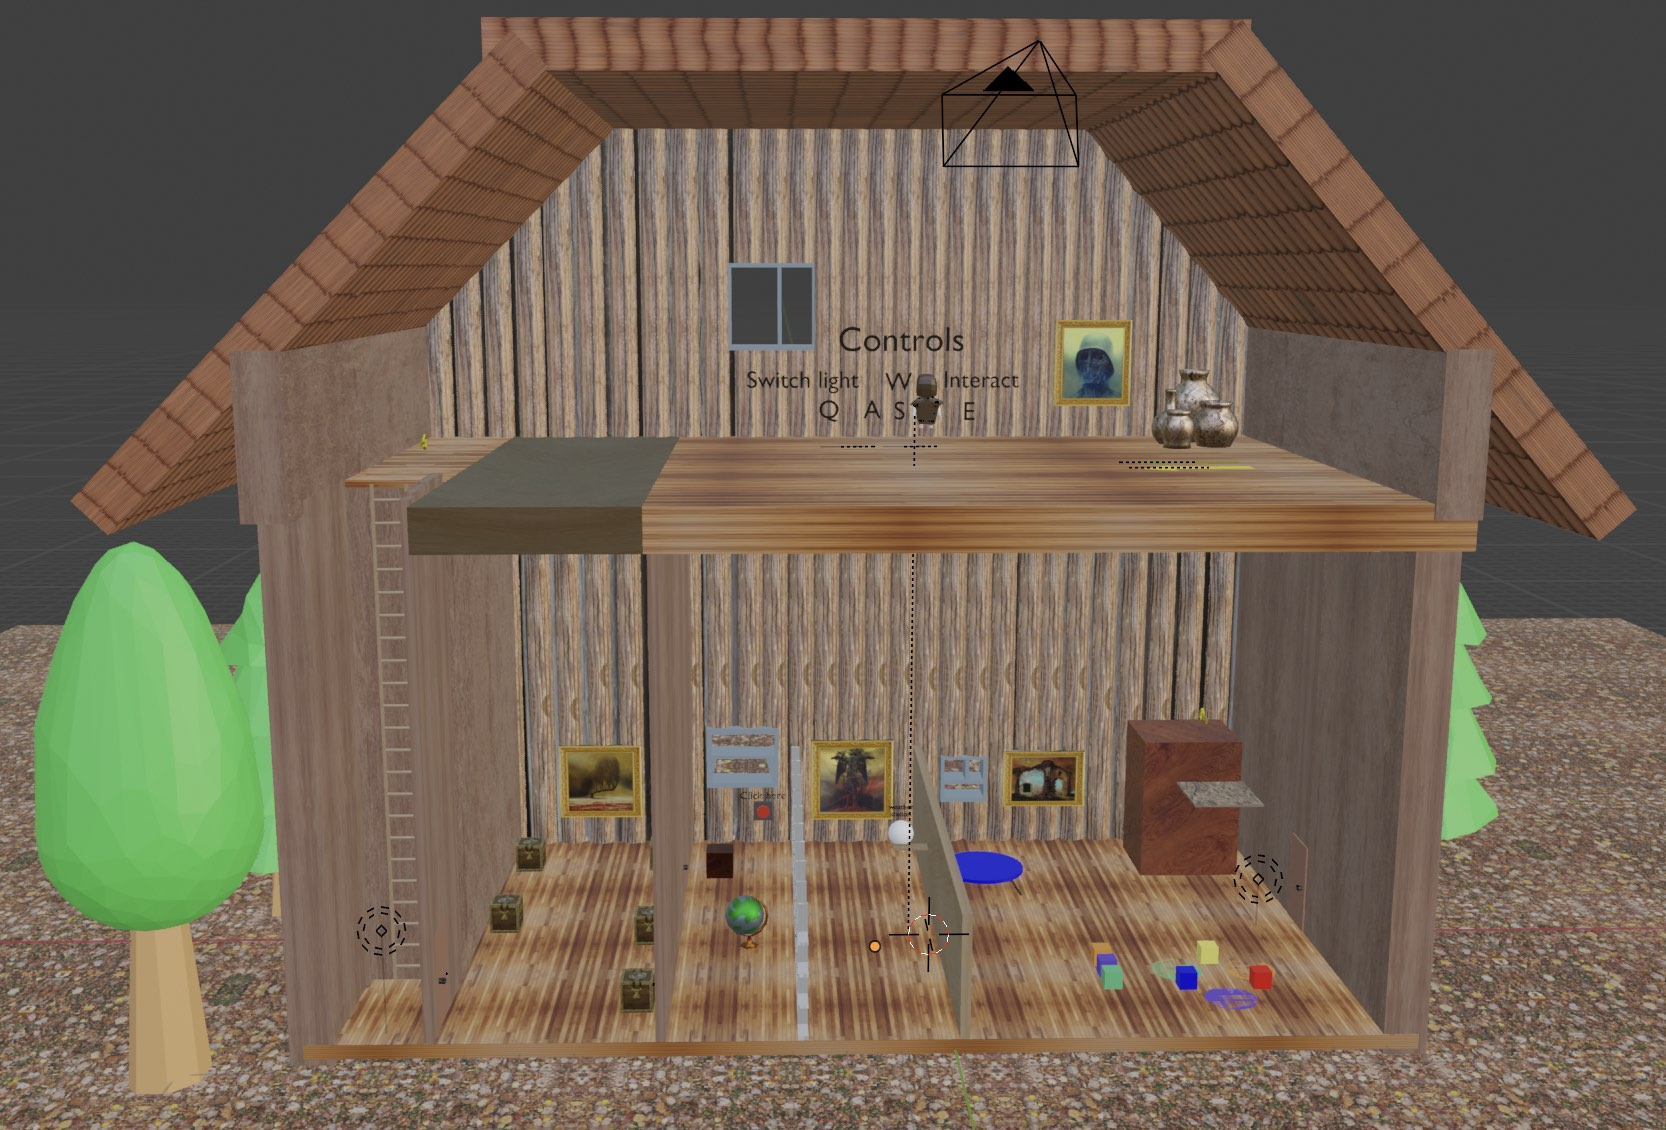
\includegraphics[width=\columnwidth]{svet.jpg}
        \caption{Celotna scena v Blenderju.}
    \end{center}
\end{figure}


Nekaj objektov, ki so v igri, smo dobili s spleta, nekatere pa smo izdelali sami. Sami smo izdelali Froda, stene, ograjo, lestev, ključ, petrolejko, trampolin in drevesa. Kompleksnejše okraske kot so vaze in globus pa smo dobili s spleta\footnote{\url{https://www.cgtrader.com/3d-models/various/various-models/viking-pots-vases-low-poly-game-ready}} \footnote{\url{https://www.cgtrader.com/free-3d-models/interior/interior-office/low-poly-world-globe}}. Vse slikovne teksture, kot so zid, kamen in les, smo prav tako pridobili s spleta\footnote{\url{https://media.freestocktextures.com/cache/12/3e/123ef654c1c7e28fafaa983956e0509e.jpg}} \footnote{\url{https://pngtree.com/freebackground/wood-grain-texture-wooden-flooring-design-with-wooden-floor-textures_12863779.html}} \footnote{\url{https://img.pikbest.com/wp/202344/wood-surface-exterior-view-of-log-house-wall-textured-and-characterful-knots_9926058.jpg!bw700}}. Za 3D modeliranje smo uporabljali program Blender, nato pa smo jih za uporabo v igri izvozili v GLTF formatu.

\subsection{Ozadje}
V ozadju se nahaja gozd, ki je prikazan tako, kot da bi bila svetu orisana kocka, na katero je prilepljena tekstura gozda (skybox), ki smo jo našli na spletu\footnote{\url{https://www.pngwing.com/en/free-png-zlcpx}}. Ta gozd sicer ni veliko viden, saj velik del zaslona zasedajo stene, ga pa lahko vidimo skozi okna hiše. Hiša je obdana s tlemi, na katerih je tekstura z listi\footnote{\url{https://cdn.materialsoftheworld.com/wp-content/uploads/2022/05/28094405/materials-of-the-world-forest-ground-leaves-render-04.jpg}}. Ostali predmeti, ki spadajo v ozadje sveta, so tudi različni okraski kot so vaze, globus in slike na stenah\footnote{\url{https://beks.pl/}}.

\begin{figure}[!htb]
    \begin{center}
        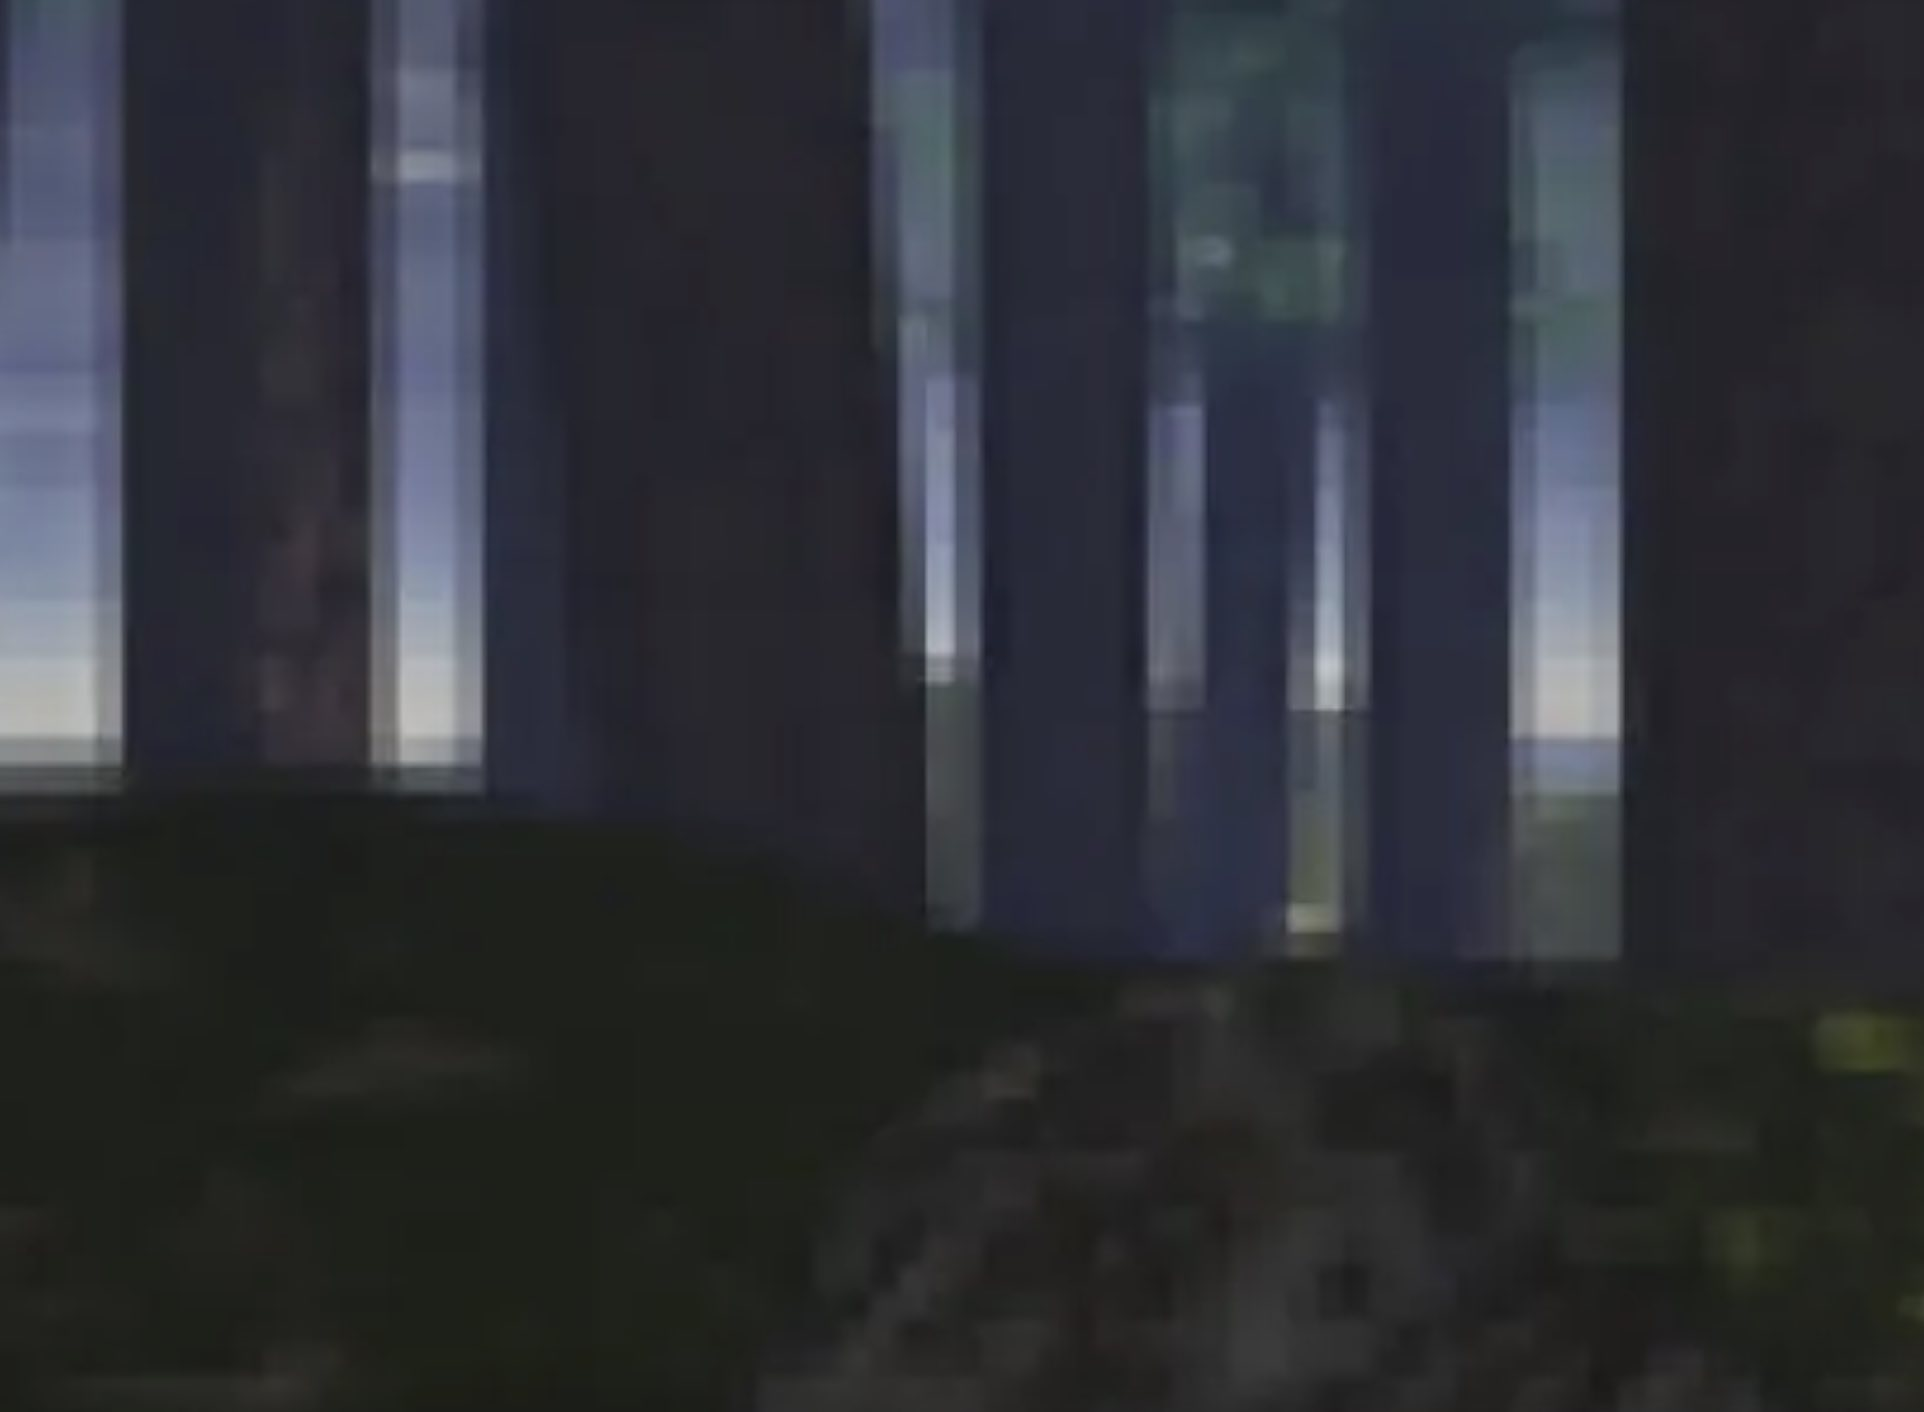
\includegraphics[width=0.8\columnwidth]{skybox.jpg}
        \caption{Izgled skyboxa v igri.}
    \end{center}
\end{figure}


V hišo smo dodali tudi kroglo, na katero se preslika skybox tekstura ozadja, tako da igralec lahko vidi, kakšno je vreme izven hiše.

\subsection{Velikost}
Igralec poleg Froda vidi še njegovo neposredno okolico. Frodo je velik približno 110 cm, kamera pa vidi približno 6 metrov širine okoli njega. Igralec interaktira z objekti, ki so približno polovični njegovi velikosti, sama hiša pa je dolga 20 m in široka 12 m.


\section{Igralni pogon in uporabljene tehnologije}
Za izdelavo igre smo uporabljali programski jezik Javascript in WebGPU vmesnik. WebGPU nam omogoča, da podatke o mrežah modelov, teksturah, lučeh, kameri in ostalo pošiljamo v grafični cevovod. Te podatke nato obdelamo v senčilnikih, ki so napisani v jeziku WebGPU Shading Language (WGSL) in tako dobimo barve pikslov na zaslonu. Pri delu smo si pomagali s knjižnico webgpu-utils\footnote{\url{https://github.com/greggman/webgpu-utils}} in s primeri iz repozitorija webgpu-examples\footnote{\url{https://github.com/UL-FRI-LGM/webgpu-examples}}.

V Javascriptu na začetku igre naložimo vse potrebne 3D modele in pripravimo grafični cevovod. Nato se za vsako sličico (frame) kliče metoda \verb+render+, ki ustrezno posodobi svet glede na trenutno stanje in vhode, ki jih je podal igralec.

Da ne pride do popačenosti tekstur, se z uporabo WebGPU ob nalaganju tekstur ustvarijo še mip map nivoji, kjer je dimenzija vsakega višjega nivoja enaka polovici prejšnjega. Za pravilno implementacijo trilinearne interpolacije smo si pomagali s knjižnico webgpu-utils.

Za zaznavanje trkov uporabljamo "axis aligned bound box"-e (AABB). Torej za vsak predmet, v katerega se lahko zaletiš, izračunamo maksimalne in minimalne točke na vsaki osi in potem za vsako sličico preverjamo ali se je uporabnik zaletel. Če se je, ga premaknemo za toliko v vsaki smeri, da ni več v trku.

V drugi sobi mora igralec z miško klikniti na model gumba v sceni. Zaznavanje, če je bil gumb pritisnjen, je izvedeno tako, da se iz mesta na zaslon, kamor je igralec kliknil, sledi žarek na sceno. Za sledenje žarka moramo koordinate klika pretvoriti iz koordinatnega sistema zaslona v koordinatni sistem sveta. Če ta žarek seka AABB gumba, se upošteva, da je bil gumb pritisnjen.

Za boljšo učinkovitost v grafični cevovod pošljemo samo oglišča modelov, ki so dejansko vidni na zaslonu. To pomeni, da na CPU predčasno izračunamo, kateri AABB-ji so v vidnem polju kamere. Na žalost to nima nobenega izmerljivega vpliva na hitrost delovanja, saj je naša scena premajhna.

\section{Pogled}
Za pogled v svet smo uporabili kamero s perspektivno projekcijo. Kamera je tretjeosebna in je postavljena tako, kot da bi gledala skozi enega izmed zidov. Ko se igralec premakne, se nad kamero izvede enaka translacija, kot nad igralcem.

Po tem ko igralec pobere ključ, je kamera nekaj časa animirana, da igralec lahko vidi, katera vrata so se odprla.

\section{Osebek}
 Glavni osebek v igri je Frodo, ki ga igralec upravlja s tipkami W (naprej), A (levo), S (dol), D (desno) in presledek (skok). Nad njim ves čas deluje gravitacija s pospeškom 20 \(m/s^{2} \). Frodo v roki drži luč, katere tip se lahko zamenja s tipko Q. Ko se Frodo dovolj približa izbranim škatlam, z njimi interaktira s tipko E. Ta lahko odpre škatlo ali pa jo premakne.
Ko se Frodo premika, se njegovo telo animira. Animacije so izvedene tako, da je njegovo telo razsekano na različne dele, ki se rotirajo s kvadratnim lajšanjem hitrosti, zaradi česar pospeški rok in nog delujejo bolj naravno.

\section{Uporabniški vmesnik}
\noindent Igro poleg glavnega platna sestavljata še dva HTML odseka. Prvi se pokaže preden se igra začne in vsebuje znak za nalaganje igre in gumb za začetek. Ko je igra zaključena, se uporabniku prikaže stran, na kateri piše, koliko časa je igralec porabil in gumb za začetek nove igre.

\section{Gameplay}
Igra se začne v zgornjem nadstropju hiše. Tam se igralec spozna s tipkami za interakcijo in vidi prve okraske. V tem nadstropju se nahaja tudi platforma, ki se podre, ko igralec stopi nanjo. Nato pride v prvo nadstropje, kjer se nahajajo tri sobe.

 V prvi sobi so postavljene škatle, ki jih igralec lahko odpira. Ko odpre pravo škatlo, dobi petrolejko in odprejo se mu vrata v naslednjo sobo. Tam se nahajajo škatla, globus, ograja in gumb za nadzor ograje. Igralec mora z miško pritisniti na gumb, ki odpre ograjo in povleči škatlo, da lahko preskoči zid do naslendje sobe. V tretji sobi se nahaja prvi ključ, do katerega pride tako, da postavi razmetane kocke na označeno mesto, kar povzroči, da se aktivira platforma, ki preko trampolina vodi do ključa. Nato lahko pride v zadnjo sobo, kjer igralca čakata še lestev in zadnji ključ.
 
Ko igralec pade na tla izven hiše (torej gre skozi izhodna vrata), se igra konča.


\begin{figure}[!htb]
    \begin{center}
        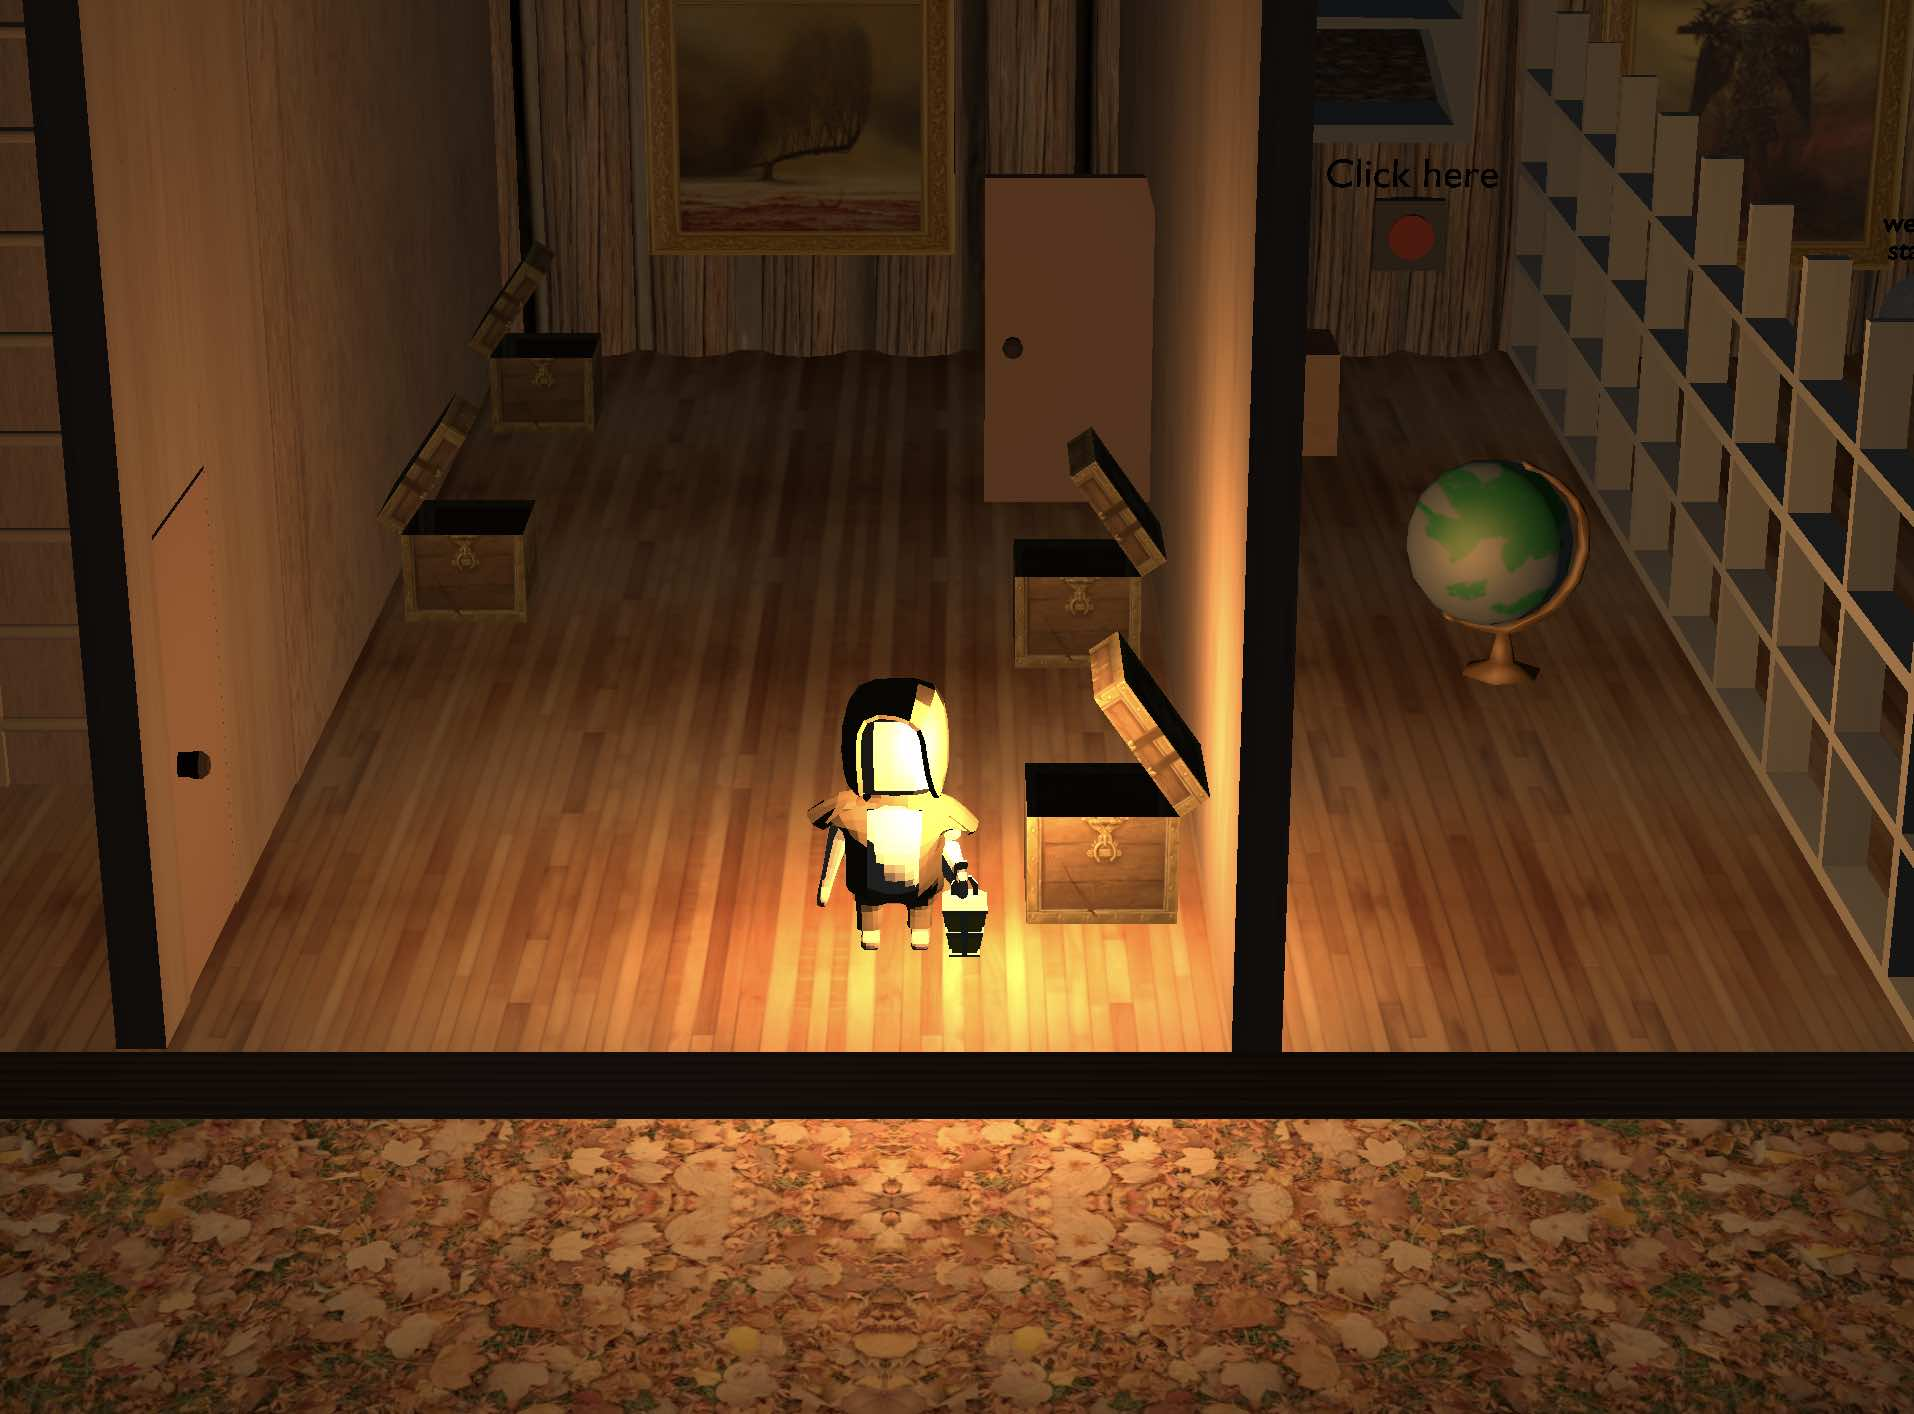
\includegraphics[width=0.9\columnwidth]{prva.jpg}
        \caption{Igra po končani prvi sobi spodnjega nadstropja.}
    \end{center}
\end{figure}

\begin{figure}[!htb]
    \begin{center}
        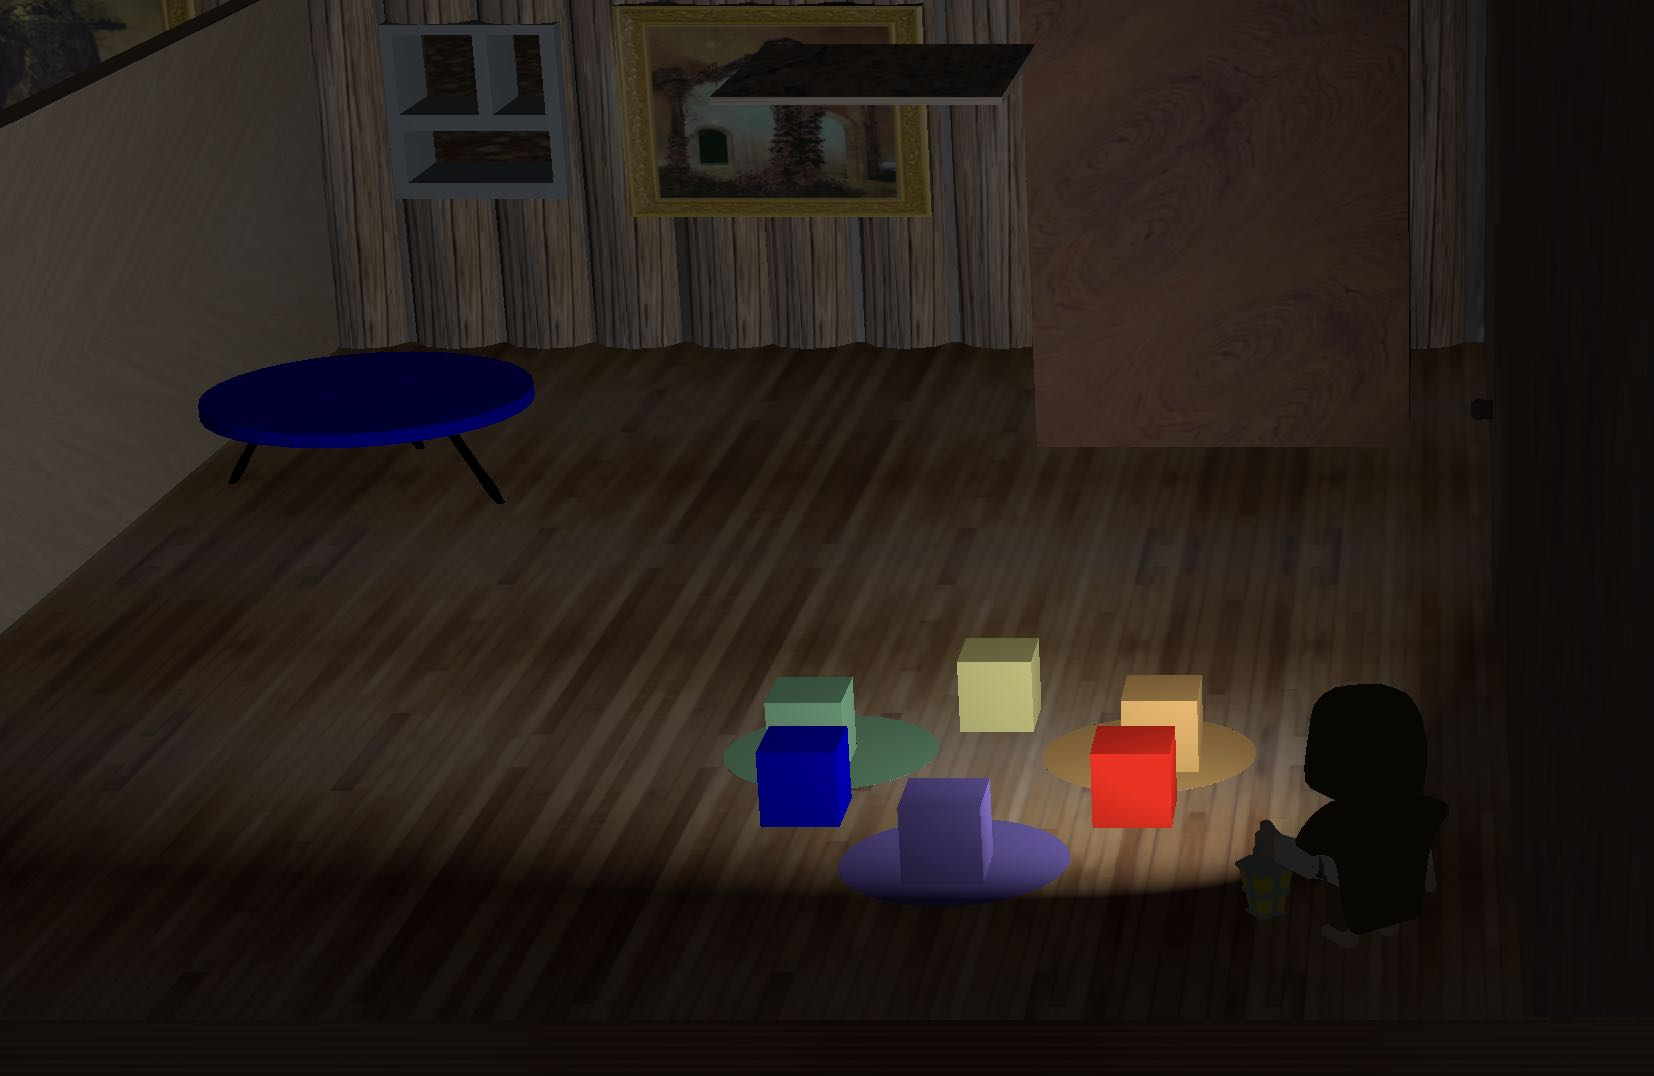
\includegraphics[width=0.9\columnwidth]{druga.jpg}
        \caption{Tretja soba z rešeno uganko in ročno svetilko kot lučjo.}
    \end{center}
\end{figure}

\newpage

\section{Luči}
V sceni so štiri luči. Prva je petrolejka, ki je izvedena kot točkovni vir svetlobe in oddaja oranžno barvo. Njena intenziteta se rahlo spreminja s časom, kar simulira plamen. Druga luč je ročna svetilka, ki je izvedena kot reflektorska luč bele barve. Prehod med osvetljenim in neosvetljenim delom je gladek, kar je izvedeno s \verb+smoothstep+ funkcijo v WGSL. Potem pa imamo še dve točkovni luči, ki osvetljujeta vrata. Te dve luči se prižgeta, ko se začne animirana kamera.
Za osvetlitveni model smo izvedli Blinn-Phongov osvetlitveni model, ki nam omogoča izvedbo neidealnega odboja na določenih predmetih. Večina objektov je takega materiala, da leska ne oddajajo, se pa opazi pri vazah, globusu in ključih.

\section{Glasba}
V ozadju se ves čas predvaja glasba, ki smo jo vzeli iz Youtube-ove glasbene knjižnice\footnote{\url{https://www.youtube.com/audiolibrary}}. Različni zvoki se predvajajo tudi, ko hodiš, skočiš in pobereš ključ. Tudi te smo vzeli s spleta\footnote{\url{https://www.zapsplat.com}}.

\section{Zaključki in možne nadgradnje}
Na začetku dela smo imeli v mislih več ugank, ampak smo se nato osredotočili samo na nekaj izbranih. Izgled igre bi lahko še izboljšali, če bi nam uspelo dodati sence v sistem osvetljevanja. Animacij s kostmi nam ni uspelo prenesti iz Blenderja v igro, tako da trenutne animacije ne izgledajo najbolj popolno. Gibanje kamere bi lahko bilo bolj gladko tako, da bi se kamera za igralcem premikala z zamikom. V igro bi lahko dodali tudi pošasti, ki bi se jim moral na poti do izhoda izogibati.
Kljub vsemu, česar nam ni uspelo dokončati v danem času, smo z rezultatom zelo zadovoljni.


\end{document}
